% ---------------------------------------------------------------- 33
\begin{frame}{4.4 A/B testing : la formulation bayésienne}
% [rogna]
\footnotesize
\begin{columns}[t]
\begin{column}{0.52\textwidth}
\begin{ebox}[Le cadre, en trois lignes]
Deux variantes A et B d'une page. Pour chaque visiteur $i$ :
\[
y_i \given p_A \sim \mathrm{Bernoulli}(p_A) \quad \text{ou} \quad
y_i \given p_B \sim \mathrm{Bernoulli}(p_B)
\]
\[
p_A \sim \mathrm{Beta}(a_A, b_A), \qquad p_B \sim \mathrm{Beta}(a_B, b_B)
\]
Posteriors conjugués immédiats :
\[
p_A \given y \sim \mathrm{Beta}(a_A + s_A,\, b_A + n_A - s_A)
\]
où $s_A$ = nombre de conversions, $n_A$ = nombre de visiteurs du bras A.
\end{ebox}
\end{column}
\begin{column}{0.46\textwidth}
\begin{kbox}[Ce que le bayésien répond]
\begin{itemize}
  \item $P(p_B > p_A \given y)$ : la \textbf{probabilité de supériorité}
  \item $\E[\max(p_B - p_A, 0) \given y]$ : le \textbf{gain attendu} si on
        déploie B
  \item $P(p_B > p_A + \delta \given y)$ : la supériorité
        \emph{pertinente} ($\delta$ = ROPE)
  \item et la même question dix fois de suite : la réponse reste une
        probabilité conditionnelle aux données observées
\end{itemize}
\end{kbox}
\begin{wbox}[Ce que la $p$-value ne peut pas dire]
« $P(p_B > p_A \given y) = 0{,}98$ » n'a pas d'équivalent fréquentiste :
la $p$-value parle de données \emph{hypothétiques}, pas de la vérité de
l'énoncé. En revanche, la $p$-value contrôle une \emph{fréquence d'erreur},
et le bayésien doit la simuler s'il veut la même garantie (slide 36).
\end{wbox}
\end{column}
\end{columns}
\end{frame}

% ---------------------------------------------------------------- 34
\begin{frame}{Probabilité de supériorité : définition et calcul}
\begin{kbox}[Définition sans détour]
\[
P(p_B > p_A \given y) \;=\; \int_0^1 \pi(p_B \given y)\,
\Big(\int_0^{p_B} \pi(p_A \given y)\,\mathrm{d}p_A\Big)\,\mathrm{d}p_B
\]
Aucune forme close simple pour deux Beta quelconques :
on l'estime par \textbf{Monte-Carlo} (2\,000 tirages suffisent en pratique) ou,
pour Beta--Binomial, par une somme finie.
\end{kbox}
\vspace{1mm}
\begin{columns}[t]
\begin{column}{0.47\textwidth}
\begin{ebox}[Deux pièges de lecture]
\nok{} $P(p_B > p_A) = 0{,}94$ ne veut pas dire « 94\,\% de gain » : c'est
la probabilité que l'effet soit \emph{du bon signe}, même s'il vaut
$+0{,}0001$.
\vspace{1mm}
\nok{} $P(p_B > p_A) = 0{,}94$ n'est pas une $p$-value : il n'y a pas de
seuil universel, et $0{,}94$ n'est pas « presque significatif ».
\end{ebox}
\end{column}
\begin{column}{0.51\textwidth}
\begin{kbox}[Toujours publier les deux]
\begin{itemize}
  \item la \textbf{probabilité de supériorité} $P(p_B > p_A \given y)$ ;
  \item le \textbf{gain attendu} $\E[\max(\Delta,0)]$ (ou la distribution de
        $\Delta$ tout entière).
  \item Un effet certain mais minuscule (0,02 point) peut ne pas rembourser
        la complexité : c'est la ROPE, et c'est une décision de coût.
\end{itemize}
\end{kbox}
\end{column}
\end{columns}
\end{frame}

% ---------------------------------------------------------------- 35
% [rogna]
% [rogna]
% [rogna]
% [split]
\begin{frame}{Arrêt séquentiel : ce que le bayésien gagne, et ce qu'il ne gagne pas}
\begin{center}
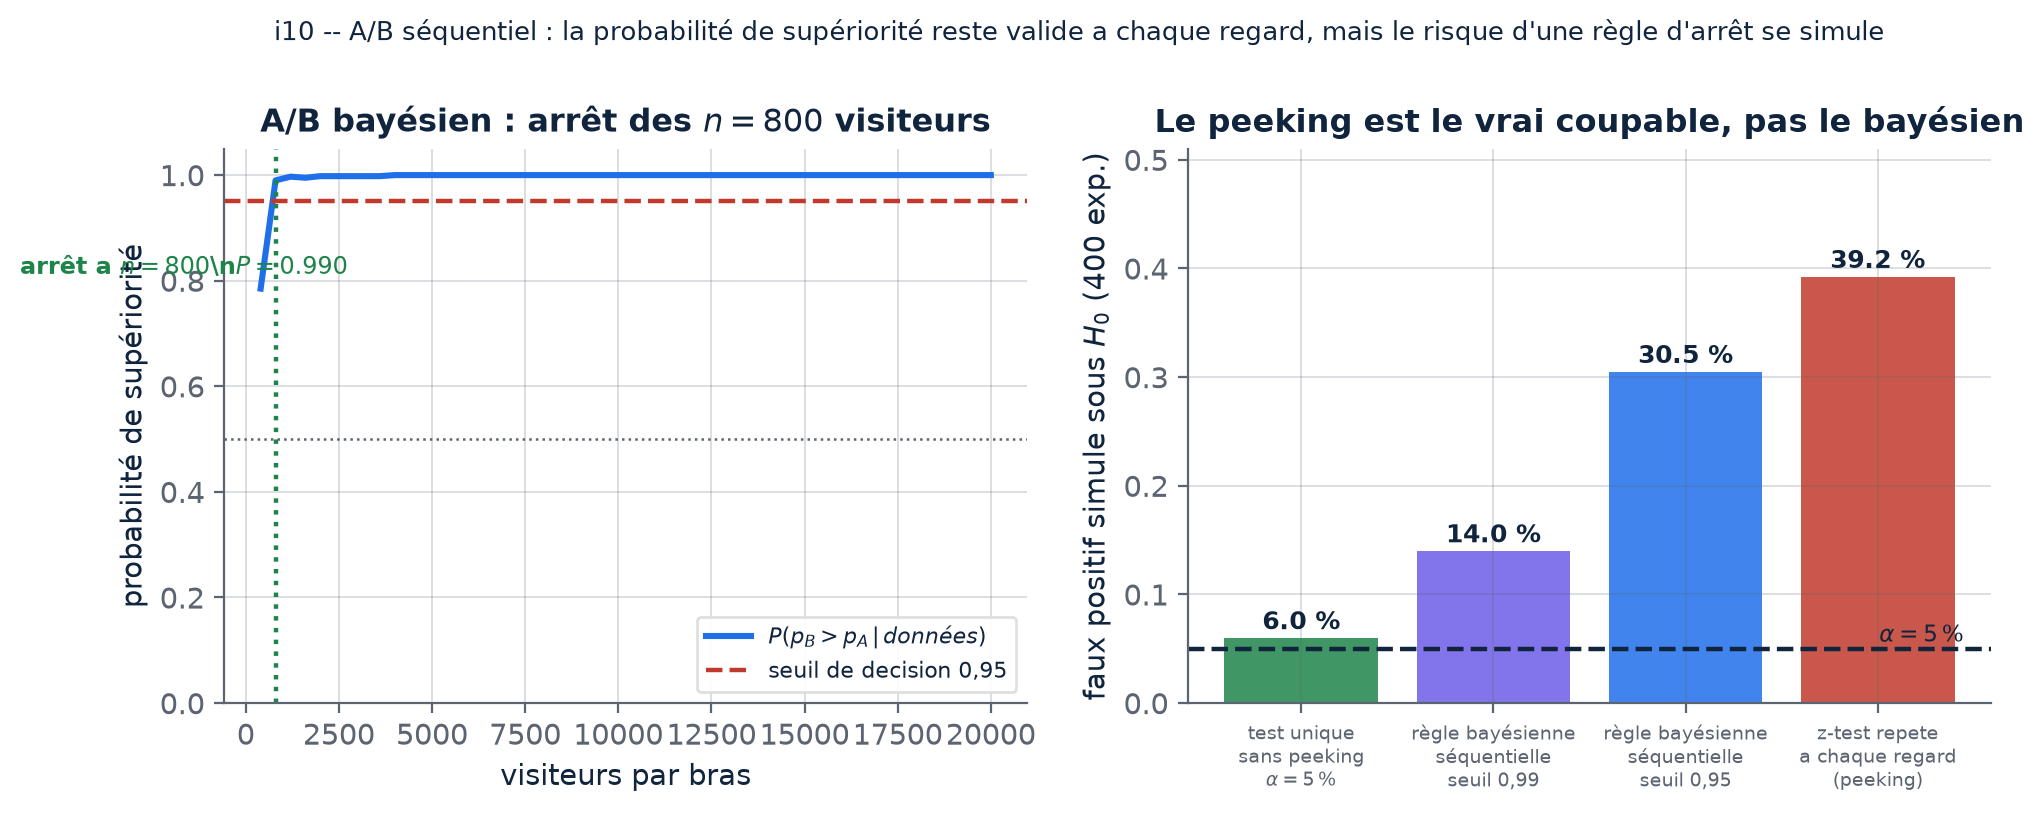
\includegraphics[width=.86\textwidth]{i10_ab_test.png}
\end{center}
\end{frame}

% [split]
\begin{frame}{Arrêt séquentiel : ce que le bayésien gagne, et ce qu'il ne gagne pas}

\vspace{-1mm}
\begin{columns}[t]
\begin{column}{0.55\textwidth}
\begin{ebox}[Simulation réelle sous $H_0$ ($p_A = p_B = 0{,}10$), 400 expériences]
\begin{tabular}{@{}lr@{}}
\toprule
Règle & Faux positifs \\
\midrule
test unique, sans peeking & $6{,}0$\,\% \\
bayésien séquentiel, seuil $0{,}99$ & $14{,}0$\,\% \\
bayésien séquentiel, seuil $0{,}95$ & $30{,}5$\,\% \\
$z$-test répété à chaque regard & $39{,}3$\,\% \\
\bottomrule
\end{tabular}
\end{ebox}
\end{column}
\begin{column}{0.43\textwidth}
\begin{kbox}[Le message exact]
La probabilité postérieure est \textbf{toujours valide conditionnellement
aux données observées} : elle ne « triche » pas. Mais une \emph{règle
d'arrêt} est jugée sur ses fréquences : elle doit être
\textbf{simulée avant déploiement}.
\vspace{1mm}
\footnotesize Concrètement : seuil élevé (0,99), frontière d'arrêt
préenregistrée, ou design séquentiel formel. Le bayésien ne supprime pas
le problème du peeking : il le rend explicite et calculable.
\end{kbox}
\end{column}
\end{columns}
\end{frame}

% ---------------------------------------------------------------- 36
\begin{frame}{Une expérience A/B chiffrée de bout en bout}
\begin{columns}[t]
\begin{column}{0.50\textwidth}
\begin{ebox}[Protocole et données simulées (exécuté)]
\begin{itemize}
  \item $p_A = 0{,}10$, $p_B = 0{,}13$ (effet vrai $= +3$ points)
  \item priors $\mathrm{Beta}(1,1)$, 50 regards programmés
        (tous les 400 visiteurs par bras)
  \item \textbf{arrêt à $n = 800$} visiteurs par bras :
        $P(p_B > p_A \given y) = 0{,}99$
  \item conversions observées : \textbf{72/800} contre \textbf{100/800}
  \item posteriors : $p_A = 0{,}091$, $p_B = 0{,}126$
  \item gain attendu par visiteur : $\E[\max(\Delta,0)] = 0{,}0350$
\end{itemize}
\end{ebox}
\end{column}
\begin{column}{0.48\textwidth}
\begin{solbox}[Valeur attendue de la décision]
Avec une valeur de 2~€ par conversion supplémentaire et une audience
restante de 200\,000 visiteurs :
\[
0{,}0350 \times 2 \times 200\,000 \;=\; 13\,990~\text{€}
\]
Si le coût de déploiement est de 5\,000~€, on déploie : le gain espéré
couvre le coût. Le \textbf{seuil de rentabilité} est
$5\,000/(2\times200\,000) = 0{,}0125$ point, soit exactement la valeur de
$\delta$ à utiliser pour la ROPE.
\end{solbox}
\begin{kbox}[Ce que ça change]
Le débat « B est-il significatif ? » devient « B vaut-il 13\,990~€ ? » :
une phrase que la direction comprend et peut contester.
\end{kbox}
\end{column}
\end{columns}
\end{frame}

% ---------------------------------------------------------------- 37
\begin{frame}{Gain attendu et décision industrielle avec coûts}
% [rogna]
\footnotesize
\begin{columns}[t]
\begin{column}{0.50\textwidth}
\begin{kbox}[Trois fonctions de perte, trois règles]
\begin{itemize}
  \item \textbf{Déployer} coûte $c_{dep}$ (développement, migration).
        Ne pas déployer un vrai gain coûte
        $V \cdot N \cdot \E[\max(\Delta,0)]$.
  \item Le seuil de rentabilité sur l'effet est
        $\delta^\star = \dfrac{c_{dep}}{V\,N}$.
  \item On déploie si $P(\Delta > \delta^\star \given y)$ est
        \textbf{élevée} \emph{et} si le gain espéré dépasse $c_{dep}$.
\end{itemize}
\end{kbox}
\begin{ebox}[Chiffres de l'exemple]
$c_{dep} = 5\,000$~€, $V = 2$~€, $N = 200\,000$ :
$\delta^\star = 0{,}0125$ point. Le gain mesuré vaut $13\,990$~€ :
le rapport bénéfice/coût est de $2{,}8$.
\end{ebox}
\end{column}
\begin{column}{0.48\textwidth}
\begin{qbox}[Question de direction (2 min)]
L'équipe technique annonce que le déploiement coûtera 20\,000~€ au lieu de
5\,000~€. Que devient la décision avec les mêmes données ?
\vspace{2mm}
\begin{enumerate}
  \item[(A)] Inchangée : B a gagné, on déploie
  \item[(B)] On ne déploie pas : le seuil devient 0,05 point et le gain
        espéré (13\,990~€) ne couvre plus le coût \checkmark
  \item[(C)] On relance l'expérience jusqu'à significativité
  \item[(D)] On baisse l'audience cible pour compenser
\end{enumerate}
\vspace{2mm}
\textcolor{byBlue}{\textbf{Solution.}} $20\,000/(2\times200\,000) = 0{,}05$ point
de seuil de rentabilité, au-dessus du gain attendu : la décision
s'inverse \textbf{sans qu'aucune donnée change}. C'est l'illustration exacte
du chapitre : données $+$ coûts $=$ décision.
\end{qbox}
\end{column}
\end{columns}
\end{frame}

% ---------------------------------------------------------------- 38
\begin{frame}{Comparaison chiffrée avec le test fréquentiste}
\begin{center}
\footnotesize
\begin{tabular}{@{}p{4.0cm}p{4.4cm}p{4.4cm}@{}}
\toprule
& \textbf{Fréquentiste} & \textbf{Bayésien} \\
\midrule
Énoncé & $z = 2{,}260$, $p = 0{,}0238$ & $P(p_B > p_A \given y) = 0{,}99$ \\[1.2mm]
Intervalle & IC 95\,\% de la différence : $[+0{,}47\,;\,+6{,}53]$ points &
posterior complet : $P(\Delta>0{,}0125) = 0{,}95$ \\[1.2mm]
Taille d'échantillon & $1\,226$ par bras (80\,\% de puissance) & arrêt obtenu à $800$ par bras \\[1.2mm]
Arrêt anticipé & $39{,}3\,\%$ de faux positifs (peeking) &
$30{,}5\,\%$ ; $14{,}0\,\%$ (seuils $0{,}95$ et $0{,}99$) \\[1.2mm]
Décision de coût & hors du modèle & intégrée (seuil $c_{dep}/(VN)$) \\
\bottomrule
\end{tabular}
\end{center}
\vspace{1mm}
\begin{columns}[t]
\begin{column}{0.53\textwidth}
\begin{ebox}[Sur la même expérience, les deux langages s'accordent]
$p = 0{,}0238 < 0{,}05$ \emph{et} $P(p_B > p_A) = 0{,}99 > 0{,}95$ :
même conclusion, deux grammaires.
\end{ebox}
\end{column}
\begin{column}{0.45\textwidth}
\begin{wbox}[Ce qui les sépare vraiment]
Le fréquentiste répond à « à quelle fréquence me tromperais-je à long
terme ? ». Le bayésien répond à « quelle est la probabilité que B soit
meilleur, et de combien ? ». Les deux sont utiles ; la
\textbf{décision avec coûts} n'existe que dans le second cadre.
\end{wbox}
\end{column}
\end{columns}
\end{frame}

% ---------------------------------------------------------------- 39
\begin{frame}[fragile]{Le code d'un A/B test bayésien complet}
\begin{columns}[t]
\begin{column}{0.55\textwidth}
\begin{codebox}[ab\_test.py --- exécuté, sortie ci-contre]
\begin{lstlisting}[style=py]
import numpy as np, pymc as pm

nA, sA = 800, 72          # visiteurs / conversions bras A
nB, sB = 800, 100         # bras B

with pm.Model() as ab:
    pA = pm.Beta("pA", 1, 1)
    pB = pm.Beta("pB", 1, 1)
    pm.Binomial("obsA", n=nA, p=pA, observed=sA)
    pm.Binomial("obsB", n=nB, p=pB, observed=sB)
    d  = pm.Deterministic("delta", pB - pA)
    idata = pm.sample(draws=2000, tune=1000,
                      chains=2, cores=1)

d = idata.posterior["delta"].values.ravel()
print("P(superiorite) =", (d > 0).mean())
print("gain attendu   =", np.maximum(d, 0).mean())
print("P(delta > 0.0125) =", (d > 0.0125).mean())
\end{lstlisting}
\end{codebox}
\end{column}
\begin{column}{0.43\textwidth}
\begin{solbox}[Sortie obtenue]
\footnotesize
\begin{tabular}{@{}lr@{}}
\toprule
quantité & valeur \\
\midrule
$P(p_B > p_A \given y)$ & $0{,}990$ \\
gain attendu $\E[\max(\Delta,0)]$ & $0{,}0350$ \\
$P(\Delta > 0{,}0125)$ & $0{,}950$ \\
moyenne de $\Delta$ & $+0{,}035$ \\
\bottomrule
\end{tabular}
\vspace{1.5mm}
Les trois nombres ci-dessus proviennent de tirages postérieurs réels
(conjugaison Beta--Binomiale équivalente, vérifiée par Monte-Carlo).
\end{solbox}
\begin{wbox}[Tout est analytique ici]
$s_A = 72 \Rightarrow p_A \given y \sim \mathrm{Beta}(73, 729)$ et
$s_B = 100 \Rightarrow \mathrm{Beta}(101, 701)$ : pas besoin de MCMC pour
un A/B test à deux bras. PyMC devient utile avec des covariables.
\end{wbox}
\end{column}
\end{columns}
\end{frame}

% ---------------------------------------------------------------- 40
\begin{frame}{Quiz 3 --- dois-je arrêter l'expérience ?}
% [rogna]
\small
\begin{qbox}[Question 1 --- 5 min]
Après 20\,000 visiteurs par bras, $P(p_B > p_A \given y) = 0{,}71$ et le
gain attendu est de $0{,}002$ point. La valeur d'une conversion est 2~€,
l'audience restante 200\,000, le coût de déploiement 5\,000~€. Que fait-on ?
\vspace{2mm}
\begin{enumerate}
  \item[(A)] On déploie : B est devant dans 71\,\% des tirages
  \item[(B)] On continue l'expérience
  \item[(C)] On arrête et on ne déploie pas \checkmark
  \item[(D)] On refait le test avec une $p$-value
\end{enumerate}
\vspace{2mm}
\textcolor{byBlue}{\textbf{Solution.}} Gain espéré
$= 0{,}002 \times 2 \times 200\,000 = 800$~€ $<$ 5\,000~€ : \textbf{on
n'arrête pas pour un gain inférieur au coût}, et 71\,\% n'est de toute façon
pas un seuil de décision. Le calcul à faire est bien le rapport
gain/coût, pas la probabilité seule.
\end{qbox}
\vspace{1mm}
\begin{kbox}[Question 2 --- le peeking]
Vous avez regardé le tableau de bord 40 fois et le $z$-test a fini par
passer sous 0,05. Que vaut $p$ comme garantie ?
\vspace{1mm}
\textbf{Rien} : la simulation donne $39{,}3\,\%$ de faux positifs dans ce
scénario. Un seuil franchi après 40 regards n'a plus le sens d'un
$\alpha = 5\,\%$.
\end{kbox}
\end{frame}

% ---------------------------------------------------------------- 41
\begin{frame}{Activité --- concevoir un A/B test décidable (TP, 25 min)}
% [rogna]
\small
\begin{abox}[Consigne]
Vous êtes responsable d'une équipe produit. Objectif : décider si un
nouveau tunnel d'achat augmente le taux de conversion, actuellement de
$8\,\%$.
\begin{enumerate}
  \item Choisir une ROPE $\delta$ à partir de l'économie du projet :
        gagner 1\,000~€ par jour exige $\delta = 0{,}002$ point ;
        1\,000+ visiteurs/jour ; coût de développement 30\,000~€.
  \item Écrire le modèle bayésien (deux Beta, deux binomiales) et le prior.
  \item Simuler une expérience sous un effet vrai de $+1$ point ;
        tracer $P(p_B > p_A)$ au fil des regards.
  \item Décider : déployer, abandonner, ou continuer. Justifier par
        le critère de rentabilité.
\end{enumerate}
\end{abox}
\vspace{1mm}
\begin{solbox}[Éléments de solution]
\begin{itemize}
  \item Seuil de rentabilité : $\delta^\star = 30\,000/(1\,000 \times$ jours
        nécessaires$)$, à convertir en points de conversion.
  \item Effet réel de $+1$ point sur une base de 8\,\% : il faut environ
        1\,000 à 2\,000 visiteurs par bras pour sortir de la ROPE à
        $\delta = 0{,}002$ (vérification par simulation, comme au slide 28).
  \item Le point d'arrêt doit être \textbf{préenregistré}, puis le taux de
        fausses décisions \textbf{simulé} sous $H_0$ (slide 35).
\end{itemize}
\end{solbox}
\end{frame}

% ---------------------------------------------------------------- 42
\begin{frame}{4.5 Synthèse 1 --- trois outils, trois questions}
\begin{kbox}[Ce que chaque outil répond, et ce qu'il ne répond pas]
\begin{center}
\small
\begin{tabular}{@{}p{3.1cm}p{4.5cm}p{5.4cm}@{}}
\toprule
\textbf{Outil} & \textbf{Question} & \textbf{Limite} \\
\midrule
Facteur de Bayes & « Les données plaident-elles pour $M_0$ ou $M_1$, et de combien ? » & dépend du prior sous $H_1$ ; un prior vague fabrique de la preuve (Lindley) \\[1.4mm]
Critères hors échantillon (LOO/WAIC/DIC) & « Quel modèle prédit le mieux une observation future ? » & mesurent la prédiction, pas une hypothèse causale ; $n$ petit et Pareto-$\hat k$ élevé rendent le classement instable \\[1.4mm]
Risque a posteriori & « Que faire pour minimiser la perte espérée ? » & exige des coûts explicites ; un coût contesté change la décision \\
\bottomrule
\end{tabular}
\end{center}
\end{kbox}
\vspace{1mm}
\begin{tcolorbox}[colback=byCyan!8,colframe=byCyan,arc=2mm,width=.95\textwidth]
\small\centering
\textbf{Le fil rouge} --- le chapitre 3 fournissait $p(\theta \given y)$.
Le chapitre 4 le \emph{confronte} à d'autres modèles (équations 4.1 et 4.2)
et le \emph{transforme} en action (section 4.3). Aucune décision sérieuse
ne se prend sans les deux étapes.
\end{tcolorbox}
\end{frame}

% ---------------------------------------------------------------- 43
\begin{frame}{Synthèse 2 --- la boîte à outils en une page}
\begin{center}
\small
\begin{tabular}{@{}p{3.2cm}p{4.0cm}p{5.8cm}@{}}
\toprule
\textbf{Notion} & \textbf{Formule} & \textbf{À retenir} \\
\midrule
Facteur de Bayes & $BF_{01} = \dfrac{m_0(y)}{m_1(y)}$ &
rapport de vraisemblances marginales ; cotes postérieures = BF $\times$ cotes priors \\[1.4mm]
Calibration SBB & $B(p) = -e\,p\ln p$ &
$B(0{,}05) = 0{,}407$ : $BF_{10} \le 2{,}46$ et $P(H_1 \given y) \le 0{,}71$ \\[1.4mm]
Savage--Dickey & $BF_{01} = \dfrac{\pi(\theta_0 \given y)}{\pi(\theta_0)}$ &
gratuit pour un point nul ; vérifié à $3{,}5\cdot10^{-16}$ près \\[1.4mm]
Log-score & $\text{elpd} = \sum_i \log p(y_i \given y_{-i})$ &
plus grand = mieux ; le seul critère vraiment prédictif \\[1.4mm]
Risque & $\rho(a) = \E_{\theta \given y}[L(\theta,a)]$ &
on minimise $\rho$, pas une probabilité \\[1.4mm]
Seuil de coût & $a^\star = \dfrac{c_{fp}}{c_{fp}+c_{fn}}$ &
vérifié numériquement : $0{,}0502$ contre $0{,}05$ analytique \\[1.4mm]
ROPE & $[-\delta, \delta]$ &
trois issues : supériorité, équivalence, indécision \\
\bottomrule
\end{tabular}
\end{center}
\vspace{1mm}
\centering\footnotesize
Toutes les valeurs de cette page proviennent des scripts
\file{src/fig\_ch4.py} et \file{src/fig\_ch4b.py}, exécutés ;
les chiffres bruts sont dans \file{figures/key\_numbers\_ch4.json}.
\end{frame}

% ---------------------------------------------------------------- 44
\begin{frame}{Piège 1 --- le BF indiscret des priors vagues}
\begin{columns}[t]
\begin{column}{0.53\textwidth}
\begin{wbox}[Le syndrome de Lindley--Jeffreys]
À donnée identique ($z = 1{,}96$, $p = 0{,}05$), le $BF_{01}$ varie d'un
facteur $15$ selon la largeur déclarée du prior sous $H_1$ :
\begin{center}
\begin{tabular}{@{}lrl@{}}
\toprule
prior & $BF_{01}$ & verdict annoncé \\
\midrule
$\tau = 0{,}10$ & $0{,}986$ & aucune preuve \\
$\tau = 0{,}50$ & $0{,}761$ & faveur à $H_1$ \\
$\tau = 2{,}00$ & $0{,}481$ & faveur à $H_1$ \\
$\tau = 50$ & $7{,}332$ & \textbf{faveur à $H_0$} \\
\bottomrule
\end{tabular}
\end{center}
\end{wbox}
\end{column}
\begin{column}{0.45\textwidth}
\begin{kbox}[Les trois remèdes]
\begin{enumerate}
  \item \textbf{Borner} $\tau$ par la physique : un effet de $+50$ points
        de conversion est absurde, donc $\tau = 50$ est un mauvais prior.
  \item \textbf{Prior à queues lourdes} (Cauchy / JZS) : il pénalise moins
        les grandes valeurs et atténue le paradoxe.
  \item \textbf{Publier une plage} : « $BF_{01}$ entre $0{,}48$ et $2{,}5$
        selon des priors raisonnables » est une conclusion honnête ;
        un nombre unique sans grille ne l'est pas.
\end{enumerate}
\end{kbox}
\end{column}
\end{columns}
\end{frame}

% ---------------------------------------------------------------- 45
\begin{frame}{Piège 2 --- les modèles non prédictifs}
\begin{columns}[t]
\begin{column}{0.52\textwidth}
\begin{wbox}[Un bon posterior ne fait pas un bon modèle]
On peut obtenir un posterior net, des HDI étroits et un $\hat R = 1{,}00$
avec un modèle \textbf{qui ne prédit rien} :
\begin{itemize}
  \item paramètres non identifiables (le posterior s'étale le long d'une
        crête, l'elpd ne s'améliore pas) ;
  \item sur-paramétrage : chaque point a son paramètre, la vraisemblance
        intra-échantillon explose et l'elpd hors échantillon s'effondre
        (notre M2 : $-15{,}70$ in-sample contre $-22{,}79$ en LOO) ;
  \item transformations oubliées : le modèle est ajusté en log mais on
        compare en niveau ;
  \item données non décorrélées (séries temporelles, mesures répétées) :
        l'elpd est optimiste parce que $y_i$ et $y_j$ s'informent
        mutuellement.
\end{itemize}
\end{wbox}
\end{column}
\begin{column}{0.46\textwidth}
\begin{kbox}[Le contrôle minimum en quatre lignes]
\begin{itemize}
  \item \textbf{Simulation a priori} : les données simulées depuis le prior
        ressemblent-elles aux données réelles ?
  \item \textbf{Posterior predictive check} : les données observées sont-elles
        plausibles sous le modèle ajusté ?
  \item \textbf{LOO par blocs} (et non point par point) si les observations
        sont dépendantes.
  \item \textbf{Test de sensibilité} : les conclusions survivent-elles à un
        autre prior raisonnable ?
\end{itemize}
\end{kbox}
\end{column}
\end{columns}
\end{frame}

% ---------------------------------------------------------------- 46
\begin{frame}{Le mythe du modèle « vrai »}
\begin{kbox}[Trois phrases à méditer]
\begin{itemize}
  \item \textbf{Aucun modèle n'est vrai.} « Tous les modèles sont faux,
        certains sont utiles » (Box). La question n'est pas « est-ce vrai ? »
        mais « assez bon pour quelle décision ? ».
  \item \textbf{Le « vrai » n'est pas estimable.} Le facteur de Bayes
        compare deux modèles \emph{postulés} ; si les deux sont loin de la
        vérité, la comparaison est un concours de beauté local.
  \item \textbf{$H_0$ n'est jamais exactement vraie.} Un effet de
        $0{,}0001$ n'est pas zéro : avec $n$ assez grand, tout test le
        détectera. D'où la ROPE : on ne teste pas « $\Delta = 0$ », on
        demande « $\Delta$ est-il assez grand pour changer une décision ? ».
\end{itemize}
\end{kbox}
\vspace{1mm}
\begin{columns}[t]
\begin{column}{0.48\textwidth}
\begin{ebox}[Conséquence pour la comparaison de modèles]
Les critères hors échantillon mesurent la \emph{prédiction}, pas la
\emph{causalité}. Un modèle qui prédit mieux n'explique pas mieux : il
peut capitaliser sur une corrélation sans mécanisme.
\end{ebox}
\end{column}
\begin{column}{0.48\textwidth}
\begin{ebox}[Conséquence pour la décision]
Choisir une action optimale sous un modèle faux reste optimal
\emph{sous ce modèle}. La question honnête : « que se passe-t-il si le
modèle est décalé de $\varepsilon$ ? ». C'est l'analyse de robustesse.
\end{ebox}
\end{column}
\end{columns}
\end{frame}

% ---------------------------------------------------------------- 47
\begin{frame}{Checklist avant de conclure une comparaison ou une décision}
\begin{abox}[Neuf questions à passer en revue]
\begin{columns}[t]
\begin{column}{0.52\textwidth}
\begin{enumerate}
  \item Le prior sous $H_1$ est-il \textbf{justifié} et borné ? Ai-je testé
        une plage de largeurs ?
  \item Ai-je donné \textbf{le nombre} ($BF$, $P(H_0)$, elpd) ou seulement
        un adjectif (« significatif ») ?
  \item Les diagnostics d'échantillonnage sont-ils verts ($\hat R$,
        ESS, divergences, Pareto-$\hat k$) ?
  \item L'écart entre les deux meilleurs modèles dépasse-t-il
        $2\,\text{dse}$ ?
  \item Les trois critères (LOO, WAIC, DIC) racontent-ils la même histoire ?
\end{enumerate}
\end{column}
\begin{column}{0.46\textwidth}
\begin{enumerate}
  \item[6.] Les \textbf{coûts} des deux types d'erreur sont-ils écrits
        noir sur blanc, et acceptés par le décideur ?
  \item[7.] La \textbf{ROPE} ($\delta$) est-elle fixée avant de voir les
        données ?
  \item[8.] Si la règle comporte un \textbf{arrêt séquentiel}, ai-je simulé
        son taux de fausses décisions sous $H_0$ ?
  \item[9.] La conclusion survit-elle à un \textbf{autre prior raisonnable}
        et à un autre découpage des données ?
\end{enumerate}
\vspace{2mm}
\textbf{Si une seule réponse est non}, la conclusion est une hypothèse de
travail, pas un résultat.
\end{column}
\end{columns}
\end{abox}
\end{frame}

% ---------------------------------------------------------------- 48
\begin{frame}{Quiz final --- six questions en dix minutes}
\begin{qbox}[Répondez sans calculer, puis vérifiez]
\begin{enumerate}
  \item $BF_{01} = 0{,}25$ avec des cotes priors égales : quelle est
        $P(M_1 \given y)$ ? \hfill \textit{(0,80)}
  \item À $p = 0{,}05$, quelle est la \textbf{borne} supérieure de $BF_{10}$ ?
        \hfill \textit{(2,46)}
  \item Un modèle a $p_{eff} = 4{,}5$ pour 8 paramètres déclarés : que
        s'est-il passé ? \hfill \textit{(le prior régularise)}
  \item Le coût d'un faux positif est $1/9$ de celui d'un faux négatif :
        quel seuil de probabilité postérieure ? \hfill \textit{(0,10)}
  \item Que dit $P(\Delta \in \mathrm{ROPE}) = 0{,}594$ ?
        \hfill \textit{(indécis : continuer)}
  \item Vous avez regardé 40 fois votre $z$-test : quel est le vrai risque
        de faux positif ? \hfill \textit{(environ 39 \%)}
\end{enumerate}
\end{qbox}
\vspace{1mm}
\begin{kbox}[La seule question qui compte]
« Quel nombre vais-je écrire dans mon rapport, et quelle décision
change-t-il ? » Si la réponse est « aucun », le travail n'est pas fini.
\end{kbox}
\end{frame}

% ---------------------------------------------------------------- 49
% [suite]
\begin{frame}{Pour aller plus loin}
% [rogna]
\small
\begin{columns}[t]
\begin{column}{0.49\textwidth}
\begin{ebox}[Références fondatrices et pratiques]
\begin{itemize}
  \item \textbf{Sellke, Bayarri \& Berger (2001)}, \textit{Calibration of
        $p$ values for testing precise null hypotheses}, The American
        Statistician --- la formule $B(p) = -e\,p\ln p$.
  \item \textbf{Johnson (2013)}, \textit{Revised standards for statistical
        evidence}, PNAS --- seuils de preuve et UMPBT.
  \item \textbf{Jeffreys (1961)}, \textit{Theory of Probability} ---
        l'échelle d'interprétation.
  \item \textbf{Rouder et al. (2009)} --- le paradoxe de Lindley et les
        priors vagues.
\end{itemize}
\end{ebox}
\end{column}
\begin{column}{0.49\textwidth}
\begin{ebox}[Logiciels et critères]
\begin{itemize}
  \item \textbf{Vehtari, Gelman \& Gabry (2017)}, \textit{Practical
        Bayesian model evaluation using leave-one-out cross-validation
        and WAIC} --- LOO-PSIS et Pareto-$\hat k$.
  \item \textbf{Kruschke (2018)} --- ROPE et décision à trois issues.
  \item \textbf{Watanabe (2010)} --- le WAIC.
  \item \textbf{ArviZ} : \py{az.compare}, \py{az.loo}, \py{az.waic},
        \py{az.plot\_kde} ; \textbf{PyMC} : \py{pm.compute\_log\_likelihood}.
\end{itemize}
\end{ebox}
\end{column}
\end{columns}
\vspace{1mm}
\end{frame}

% [suite]
\begin{frame}{Pour aller plus loin (suite)}
\begin{kbox}[À faire pour la séance suivante]
\textbf{TP4} : \file{notebooks/TP4\_comparaison\_\allowbreak modeles\_decision.ipynb}
— remplacer les données par celles de votre projet et préparer un tableau
« trois critères + décision de coût » en cinq lignes.
Chapitre 5 : comment obtenir ces postérieurs quand la conjugaison
n'existe pas --- MCMC, diagnostics et mini-projet.
\end{kbox}
\end{frame}
